
\documentclass{beamer}
\mode<presentation>
\usepackage{amsmath}
\usepackage{amssymb}
%\usepackage{advdate}
\usepackage{graphicx}
\graphicspath{{../figs/}}
\usepackage{adjustbox}
\usepackage{subcaption}
\usepackage{enumitem}
\usepackage{multicol}
\usepackage{mathtools}
\usepackage{listings}
\usepackage{url}
\def\UrlBreaks{\do\/\do-}
\usetheme{Boadilla}
\usecolortheme{lily}
\setbeamertemplate{footline}
{
  \leavevmode%
  \hbox{%
  \begin{beamercolorbox}[wd=\paperwidth,ht=2.25ex,dp=1ex,right]{author in head/foot}%
    \insertframenumber{} / \inserttotalframenumber\hspace*{2ex} 
  \end{beamercolorbox}}%
  \vskip0pt%
}
\setbeamertemplate{navigation symbols}{}
\let\solution\relax
\usepackage{gvv}
\lstset{
%language=C,
frame=single, 
breaklines=true,
columns=fullflexible
}

\numberwithin{equation}{section}
\title{5.2.68}
\author{AI25BTECH11001 - ABHISEK MOHAPATRA}
% \maketitle
% \newpage
% \bigskip
\begin{document}
{\let\newpage\relax\maketitle}
\renewcommand{\thefigure}{\theenumi}
\renewcommand{\thetable}{\theenumi}




	 	\textbf{Question}:
		Solve $2x + 3y = 11$ and $2x + 4y = -24$ and hence find the value of $m$ fror which $y = mx + 3$.

		\textbf{Solution:}
		Given:
		\begin{align}
				2x +3y = 11
		\end{align},
		\begin{align}
				2x + 4y = -24
		\end{align}And,
		\begin{align}
		y = mx+3
		\end{align}
		So,
		\begin{align}
				\myvec{ 2 &3\\2&4\\m&-1}\vec{X} = \myvec{11 \\ -24\\-3}
		\end{align}
		

		Augumented Matrix:
		\begin{align}
				\augvec{2}{1}{2 & 3 & 11\\2&4&-24\\m&-1&-3}
		\end{align}
		\begin{align}
				\xrightarrow[]{R_2\rightarrow R_2-R_1}\augvec{2}{1}{2 & 3 & 11\\0&1&-35\\m&-1&-3}
		\end{align}
		\begin{align}
				\xrightarrow[]{R_3\rightarrow R_3-\frac{m}{2}R_1}\augvec{2}{1}{2 & 3 & 11\\0&1&-35\\0&-1-\frac{3m}{2}&-3-\frac{11m}{2}}
		\end{align}
		\begin{align}
				\xrightarrow[]{R_3\rightarrow R_3+(1+\frac{3m}{2})R_2}\augvec{2}{1}{2 & 3 & 11\\0&1&-35\\0&0&-38-\frac{116m}{2}}
		\end{align}
		for solution to exist the rank must be 2.
		\begin{align}
				-38 -\frac{116}{2}m = 0 \Rightarrow 58m = -38 \Rightarrow m = -\frac{19}{29}
		\end{align}

		So, m = $-\frac{19}{29}$.


Graph:
\begin{figure}[h!]
	\centering
	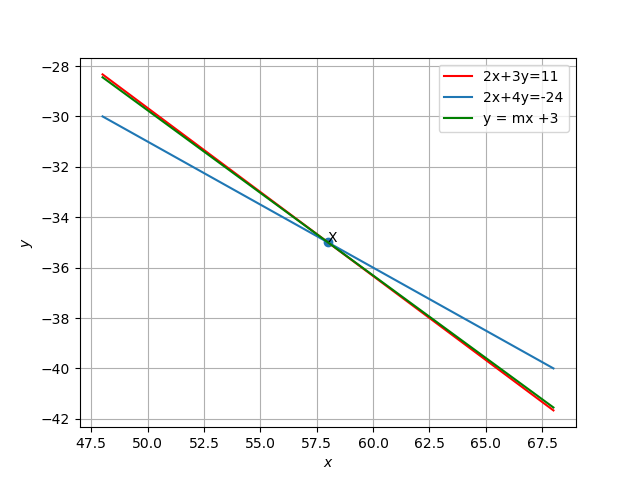
\includegraphics[width=\linewidth]{img.png}
\end{figure}	
\end{document}


